% asset_id: AS2ModellingInMechanicsTIKZ-006
\documentclass[tikz,border=8pt]{standalone}
\usepackage{amsmath}
\usetikzlibrary{positioning}
\begin{document}
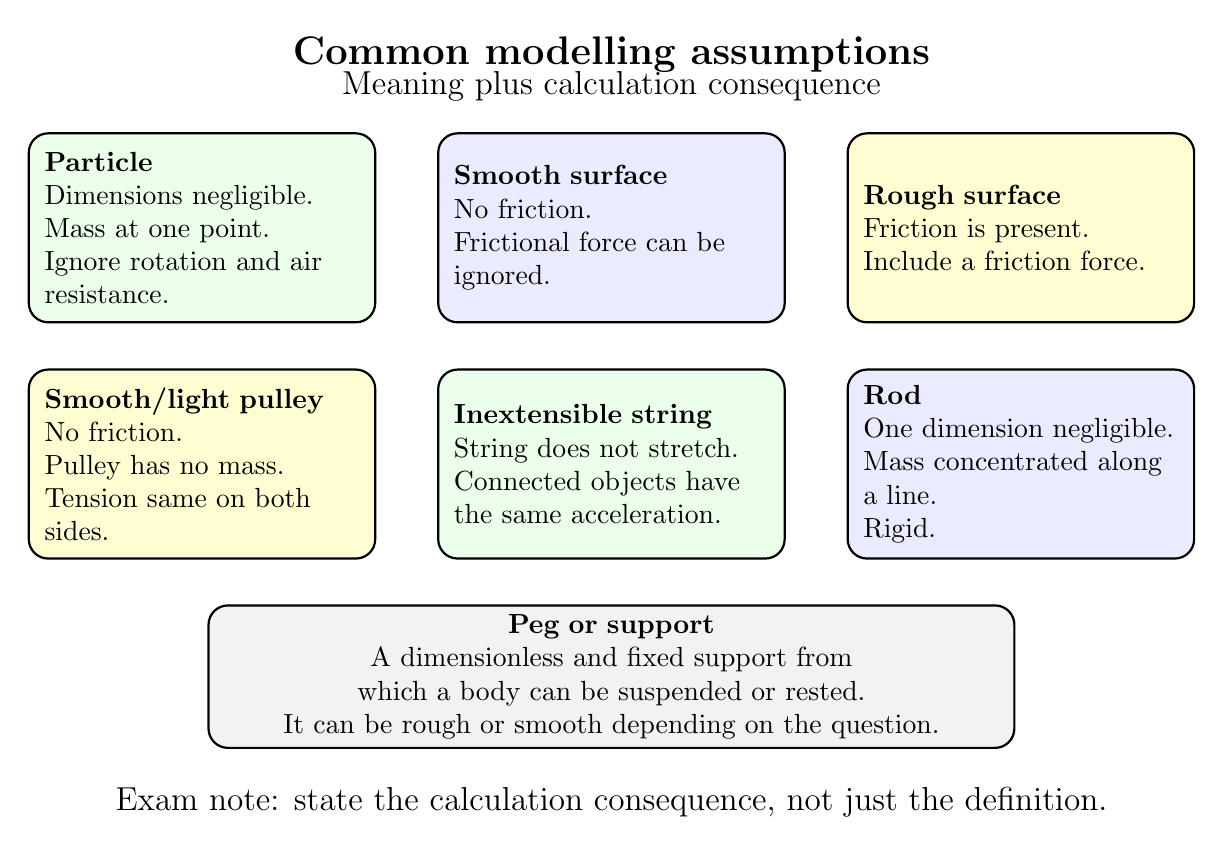
\begin{tikzpicture}[card/.style={draw, rounded corners=7pt, thick, minimum width=4.4cm, minimum height=2.4cm, align=left, text width=4.0cm}]
\node[font=\Large\bfseries] at (0,4.5) {Common modelling assumptions};\node[font=\large] at (0,4.1) {Meaning plus calculation consequence};
\node[card, fill=green!8] at (-5.2,2.3) {\textbf{Particle}\\Dimensions negligible.\\Mass at one point.\\Ignore rotation and air resistance.};\node[card, fill=blue!8] at (0,2.3) {\textbf{Smooth surface}\\No friction.\\Frictional force can be ignored.};\node[card, fill=yellow!18] at (5.2,2.3) {\textbf{Rough surface}\\Friction is present.\\Include a friction force.};\node[card, fill=yellow!18] at (-5.2,-0.7) {\textbf{Smooth/light pulley}\\No friction.\\Pulley has no mass.\\Tension same on both sides.};\node[card, fill=green!8] at (0,-0.7) {\textbf{Inextensible string}\\String does not stretch.\\Connected objects have the same acceleration.};\node[card, fill=blue!8] at (5.2,-0.7) {\textbf{Rod}\\One dimension negligible.\\Mass concentrated along a line.\\Rigid.};\node[draw, rounded corners=7pt, thick, fill=gray!10, align=center, text width=10cm] at (0,-3.4) {\textbf{Peg or support}\\A dimensionless and fixed support from which a body can be suspended or rested.\\It can be rough or smooth depending on the question.};\node[font=\large] at (0,-5.0) {Exam note: state the calculation consequence, not just the definition.};
\end{tikzpicture}
\end{document}
